\documentclass[journal,12pt,twocolumn]{IEEEtran}

\usepackage{setspace}
\usepackage{gensymb}
\singlespacing
\usepackage[cmex10]{amsmath}

\usepackage{amsthm}

\usepackage{mathrsfs}
\usepackage{txfonts}
\usepackage{stfloats}
\usepackage{bm}
\usepackage{cite}
\usepackage{cases}
\usepackage{subfig}

\usepackage{longtable}
\usepackage{multirow}

\usepackage{enumitem}
\usepackage{mathtools}
\usepackage{steinmetz}
\usepackage{tikz}
\usepackage{circuitikz}
\usepackage{verbatim}
\usepackage{tfrupee}
\usepackage[breaklinks=true]{hyperref}
\usepackage{graphicx}
\usepackage{tkz-euclide}

\usetikzlibrary{calc,math}
\usepackage{listings}
    \usepackage{color}                                            %%
    \usepackage{array}                                            %%
    \usepackage{longtable}                                        %%
    \usepackage{calc}                                             %%
    \usepackage{multirow}                                         %%
    \usepackage{hhline}                                           %%
    \usepackage{ifthen}                                           %%
    \usepackage{lscape}     
\usepackage{multicol}
\usepackage{chngcntr}

\DeclareMathOperator*{\Res}{Res}

\renewcommand\thesection{\arabic{section}}
\renewcommand\thesubsection{\thesection.\arabic{subsection}}
\renewcommand\thesubsubsection{\thesubsection.\arabic{subsubsection}}

\renewcommand\thesectiondis{\arabic{section}}
\renewcommand\thesubsectiondis{\thesectiondis.\arabic{subsection}}
\renewcommand\thesubsubsectiondis{\thesubsectiondis.\arabic{subsubsection}}


\hyphenation{op-tical net-works semi-conduc-tor}
\def\inputGnumericTable{}                                 %%
\makeatletter
\setlength{\@fptop}{0pt}
\makeatother
\lstset{
%language=C,
frame=single, 
breaklines=true,
columns=fullflexible
}
\begin{document}

\newcommand{\BEQA}{\begin{eqnarray}}
\newcommand{\EEQA}{\end{eqnarray}}
\newcommand{\define}{\stackrel{\triangle}{=}}
\bibliographystyle{IEEEtran}
\raggedbottom
\setlength{\parindent}{0pt}
\providecommand{\mbf}{\mathbf}
\providecommand{\pr}[1]{\ensuremath{\Pr\left(#1\right)}}
\providecommand{\qfunc}[1]{\ensuremath{Q\left(#1\right)}}
\providecommand{\sbrak}[1]{\ensuremath{{}\left[#1\right]}}
\providecommand{\lsbrak}[1]{\ensuremath{{}\left[#1\right.}}
\providecommand{\rsbrak}[1]{\ensuremath{{}\left.#1\right]}}
\providecommand{\brak}[1]{\ensuremath{\left(#1\right)}}
\providecommand{\lbrak}[1]{\ensuremath{\left(#1\right.}}
\providecommand{\rbrak}[1]{\ensuremath{\left.#1\right)}}
\providecommand{\cbrak}[1]{\ensuremath{\left\{#1\right\}}}
\providecommand{\lcbrak}[1]{\ensuremath{\left\{#1\right.}}
\providecommand{\rcbrak}[1]{\ensuremath{\left.#1\right\}}}
\theoremstyle{remark}
\newtheorem{rem}{Remark}
\newcommand{\sgn}{\mathop{\mathrm{sgn}}}
\providecommand{\abs}[1]{\vert#1\vert}
\providecommand{\res}[1]{\Res\displaylimits_{#1}} 
\providecommand{\norm}[1]{\lVert#1\rVert}
%\providecommand{\norm}[1]{\lVert#1\rVert}
\providecommand{\mtx}[1]{\mathbf{#1}}
\providecommand{\mean}[1]{E[ #1 ]}
\providecommand{\fourier}{\overset{\mathcal{F}}{ \rightleftharpoons}}
%\providecommand{\hilbert}{\overset{\mathcal{H}}{ \rightleftharpoons}}
\providecommand{\system}{\overset{\mathcal{H}}{ \longleftrightarrow}}
	%\newcommand{\solution}[2]{\textbf{Solution:}{#1}}
\newcommand{\solution}{\noindent \textbf{Solution: }}
\newcommand{\cosec}{\,\text{cosec}\,}
\providecommand{\dec}[2]{\ensuremath{\overset{#1}{\underset{#2}{\gtrless}}}}
\newcommand{\myvec}[1]{\ensuremath{\begin{pmatrix}#1\end{pmatrix}}}
\newcommand{\mydet}[1]{\ensuremath{\begin{vmatrix}#1\end{vmatrix}}}
\numberwithin{equation}{subsection}
\makeatletter
\@addtoreset{figure}{problem}
\makeatother
\let\StandardTheFigure\thefigure
\let\vec\mathbf
\renewcommand{\thefigure}{\theproblem}
\def\putbox#1#2#3{\makebox[0in][l]{\makebox[#1][l]{}\raisebox{\baselineskip}[0in][0in]{\raisebox{#2}[0in][0in]{#3}}}}
     \def\rightbox#1{\makebox[0in][r]{#1}}
     \def\centbox#1{\makebox[0in]{#1}}
     \def\topbox#1{\raisebox{-\baselineskip}[0in][0in]{#1}}
     \def\midbox#1{\raisebox{-0.5\baselineskip}[0in][0in]{#1}}
\vspace{3cm}
\title{Assignment 6}
\author{Ananthoju Pranav Sai - AI20BTECH11004}
\maketitle
\newpage
\bigskip
\renewcommand{\thefigure}{\theenumi}
\renewcommand{\thetable}{\theenumi}
Download all python codes from 
\begin{lstlisting}
https://github.com/Ananthoju-Pranav-Sai/AI1103/tree/main/Assignment_6/Codes
\end{lstlisting}
%
and latex codes from 
%
\begin{lstlisting}
https://github.com/Ananthoju-Pranav-Sai/AI1103/blob/main/Assignment_6/main.tex
\end{lstlisting}
\section*{GATE 1997 MA -Problem 8}
    Find the characteristic function of $Y=\sum_{r=1}^{n}a_rX_r$, where $a_1,a_2,...,a_n$ are constants and $X_1,X_2,X_3,..,X_n$ are random variables, each of which takes the values -1 and 1 with probability $\frac{1}{2}$. Taking $a_r=2^{-r}$ for each $r$, show that $Y$ converges in distribution to uniform distribution on (-1,1).
   
\section*{Solution}
Given,
\begin{align}
    Y&=\sum_{r=1}^{n}a_rX_r
\end{align}
The characteristic function of a random variable Y is defined as
\begin{align}
    C_{Y}\brak{t}&=E[e^{itY}\\
    \implies C_{Y}\brak{t}&=E[e^{it\sum_{r=1}^{n}a_rX_r}]\\
    \implies C_{Y}\brak{t}&=\prod_{r=1}^{n}E[e^{ita_rX_r}]\\
    \implies C_{Y}\brak{t}&=\prod_{r=1}^{n}C_{X_r}\brak{a_rt}
\end{align}
By taking $a_r=2^{-r}$ we get,
\begin{align}
    C_{Y}\brak{t}&=\prod_{r=1}^{n}C_{X_r}\brak{\frac{t}{2^r}}
    \label{a}
\end{align}
As random variables $X_r's$ follow discrete uniform distribution with only two possible outcomes ($X_r=-1$ and $X_r=1$) the characteristic equation of $X_r$ is
\begin{align}
    C_{X_r}\brak{t}&=\sum_{k}e^{ikt}\pr{X_r=k}\\
    \implies C_{X_r}\brak{t}&=\frac{e^{-it}}{2}+\frac{e^{it}}{2}\\
    \implies C_{X_r}\brak{t}&=\frac{1+e^{2it}}{2e^{it}}\\
    \implies C_{X_r}\brak{\frac{t}{2^r}}&=\frac{1+e^{2i\brak{\frac{t}{2^r}}}}{2e^{i\brak{\frac{t}{2^r}}}}
        \label{b}
\end{align}
using \eqref{b} in \eqref{a}
\begin{align}
    C_{Y}\brak{t}&=\prod_{r=1}^{n}\brak{\frac{1+e^{2i\brak{\frac{t}{2^r}}}}{2e^{i\brak{\frac{t}{2^r}}}}}\\
    \implies C_{Y}\brak{t}&=\frac{\brak{1+e^{it}}\brak{1+e^{i\brak{\frac{t}{2}}}}....\brak{1+e^{i\brak{\frac{t}{2^{n-1}}}}}}{2^n\brak{e^{i\sum_{r=1}^n\frac{t}{2^r}}}}\\
     \therefore C_{Y}\brak{t}&=\frac{\brak{e^{2it}-1}}{2^ne^{it\brak{\frac{2^{n+1}-1}{2^{n+1}}}}\brak{e^{\brak{\frac{it}{2^{n-1}}}}-1}}
     \label{c}
\end{align}
Now consider
\begin{align}
     \lim_{n\to\infty} C_{Y}\brak{t}\\
    \implies \lim_{n\to\infty}\frac{\brak{e^{2it}-1}}{2^ne^{it\brak{\frac{2^{n+1}-1}{2^{n+1}}}}\brak{e^{\brak{\frac{it}{2^{n-1}}}}-1}}
    \label{d}
\end{align}
We know that,
\begin{align}
    \lim_{n\to\infty}\brak{e^{\brak{\frac{it}{2^{n-1}}}}-1} &= \frac{it}{2^{n-1}}
    \label{e}\\
    \lim_{n\to\infty}e^{it\brak{\frac{2^{n+1}-1}{2^{n+1}}}}&=e^{it}
    \label{f}
\end{align}
Using \eqref{e} and \eqref{f} in \eqref{d}
\begin{align}
    \lim_{n\to\infty} C_{Y}\brak{t}&=\frac{\brak{e^{2it}-1}}{2ite^{it}}
    \label{g}
\end{align}
Now, let's assume that if $Y$ follows uniform distribution on (-1,1) then it's pdf can be written as
\begin{align}
    f_{Y}(y)=\begin{cases} 
            \frac{1}{2}  &  -1\le y\le 1\\
            0 &  otherwise
            \end{cases}
\end{align}
And it's cdf would be
\begin{align}
    F_{Y}(y)=\begin{cases} 
            0 & y<-1\\
            \frac{1+y}{2}  &  -1\le y\le 1\\
            1 &  otherwise
            \end{cases}
\end{align}
It's characteristic function would be 
\begin{align}
   C_{Y}\brak{t}&= \int_{-\infty}^{\infty} e^{ity}.f_{Y}(y) \,dy\\
    \implies C_{Y}\brak{t}&=\int_{-1}^{1} e^{ity}.\brak{\frac{1}{2}} \,dy\\
    \implies C_{Y}\brak{t}&=\frac{\brak{e^{2it}-1}}{2ite^{it}}
    \label{h}
\end{align}
So from \eqref{g} and \eqref{h} we conclude that as $\brak{n\rightarrow\infty}$ $Y$ converges in distribution to uniform distribution on (-1,1).
\begin{figure}[h]
    \centering
    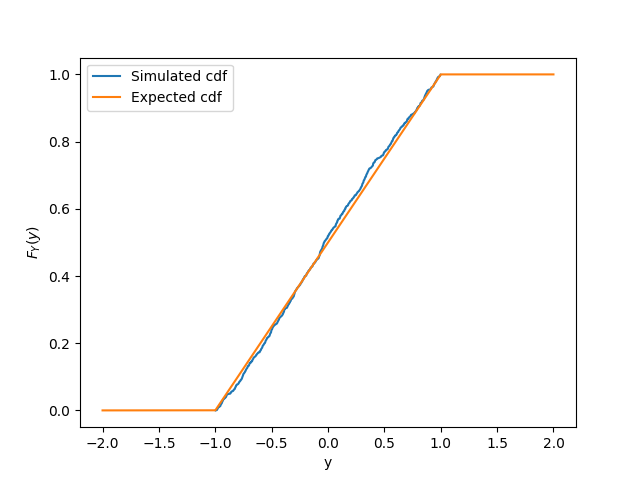
\includegraphics[width=\linewidth]{simulated_cdf.png}
    \caption{Simulated vs expected cdf plot of random variable Y}
    \label{cdf_plot}
\end{figure}
\end{document}